\section{Tales from the Anima}

\begin{quotex}

\textbf{Sehnsucht} is the inconsolable longing in the heart for we know not what. … [It is] that unnameable something, desire for which pierces us like a rapier at the smell of bonfire, the sound of wild ducks flying overhead, the title of \emph{The Well at the World's End}, the opening lines of \emph{Kubla Khan}, the morning cobwebs in late summer, or the noise of falling waves. \flright{\textsc{C S Lewis}}

You know that you love someone when you have glimpsed in her something too beautiful to die. \flright{\textsc{Gabriel Marcel}}

Ye who believe in affection that hopes, and endures, and is patient,

Ye who believe in the beauty and strength of woman's devotion,

List to the mournful tradition still sung by the pines of the forest;

List to a Tale of Love in Acadie, home of the happy. \flright{\textsc{Henry Wadsworth Longfellow}, \emph{Evangeline}}

\end{quotex}
Last night, I had another in a long series of dreams about the Anima. Our lovemaking was so sweet and enduring that we even spent time together afterwards; that is atypical. I even saw her face, which I had never clearly seen before. She was cute and somewhat petite. After three days together, I asked her if it was too soon to discuss marriage. Never before had marriage ever come up in a dream conversation. It was so disappointing to awaken. I never heard her answer.

\paragraph{Arabian Nights}
An unknown friend just sent me by post the tales of the 1001 Nights, but he neglected to send me a woman as creative as Scheherazade to read them to me. The stories have an urgency, when you consider that they represent a matter of life and death. Now I wonder what it would be like to spend 1001 nights with such a woman.

\begin{wrapfigure}{rt}{.3\textwidth}
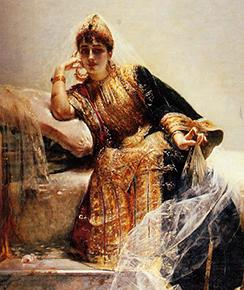
\includegraphics[scale=.5]{a20201115TalesfromtheAnima-img001.jpg} 
\caption{Scheherazade}
\end{wrapfigure}

Fearful that she would be unfaithful to him, the King married a new virgin every day, only to have her beheaded the next morning. Eventually, the kingdom ran out of virgins. The vizier's daughter, Scheherazade, volunteered to be the king's bride, to her father's consternation. But Scheherazade was quite intelligent and cultured. She had read widely in history, poetry, philosophy, science, and the arts. So on their first night together, she told the king a story, but did not finish it. Curious to hear the ending, he kept her a second night. Scheherazade finished the first story and started a second, again without finishing it. This continued for 1001 nights, at which point he admitted that he had fallen in love with her and spared her life.

Esoterically, Scheherazade risks her personal life to gain her immortal life with the king.

\paragraph{Worthiness of Love}
Frithjof Schuon points out that, according to an Hadith, \textbf{women, perfumes, and prayer} are worthy of love. Schuon explains why:

\begin{itemize}
\item \textbf{Woman}, synthesizing in her substance virgin nature, the sanctuary and spiritual company, is for man what is most lovable; in her highest aspect, she is the formal projection of merciful and infinite Inwardness in the outward; and in this regard she assumes a quasi-sacramental and liberating function. 
\item \textbf{Perfumes} represent qualities or beauties that are formless, exactly in the same way as music; that is to say that side by side with the formal projection of Inwardness, there exists also a complementary formless projection, symbolized, not by visual or tangible qualities, but by auditory and olfactory ones; perfumes are silent music. 
\item \textbf{Prayer} leads from Outward to Inward, and both consecrates and transmutes the qualitative elements of the outward realm. 
\end{itemize}

\paragraph{My Imaginary Friend}
\begin{quotex}
There is only one her for each him. She has been singled out for him in each register of the universe. This cannot be changed because She is the Her who came out of Him. In the turning of the wheel of the Eternal Return, it is not always given for them to meet. One or other may arrive late or too early.

It should be known that, in reality, the solution is to be able to bring Her back to life, to resurrect her within his soul. \flright{\textit{Nos}}

\end{quotex}
Often impatient with the all too slow process, through dreams, of the revelation of Her, I take it upon myself to imagine Her through my own efforts. But the imagination cannot create ex nihilo, so it needs an inspiration to kick it off. There are some women who are so beautiful, that men may be affected physically just by gazing upon her. This is how \textbf{Dante} described Beatrice in \emph{La Vita Nuova}:

\begin{quotex}
she showed herself so gentle and so full of all perfection, that she bred in those who looked upon her a soothing quiet beyond any speech; neither could any look upon her without sighing immediately. 

\end{quotex}
Yet even the Girl from Ipanema made the men sigh whenever she passed by. So my imagination requires more, much more. Beatrice, for Dante, represented, not just Beauty, but, more importantly, Wisdom. She guides him through the heavenly spheres toward God, something which the philosophers could not do.

Beyond a physical sigh, there is a spiritual sigh. Like Scheherazade, the image would be someone of high intellect, familiar with “history, poetry, philosophy, science, and the arts”; she would understand the transcendent meaning behind the appearances, often described in terms of the archetypes of the gods and goddesses.

And she is passionate about her life. She is elegant with refined tastes in fashion, art, architecture, perfumes. She intuitively grasps the rhythms of life, knowing when to dance and when to be still, just contemplating the world around her.

She seems to be how I might imagine myself to be, were I a woman.

\paragraph{The Soul of a Woman}
Although a woman longs to be “known”, for a man to “get her”, she nevertheless keeps many things hidden. She will drop a clue from time to time, and these must be carefully attended to. Yet the more you penetrate, and the more you think you know, something is still off kilter. It is not like looking through a window, but rather “through” a mirror. Left becomes right, and right becomes left, which is disorientating long before you become fully aware of it.

Yet it is necessary, because a man's soul is deficient. A human being consists of the physical along with the three soul functions of Willing, Feeling, and Thinking. A man focuses on his physical prowess and intellectual skills, the two least permanent parts of the human being. The physical is left behind at death along with most of one's thoughts. Thoughts have no permanent value. Even such a master of thinking like Thomas Aquinas came to the realization that they are just “so much straw”. What you Will and what you deeply Feel (not feelings in the trivial sense used by the modern world), will follow you, so these faculties also need development.

A child comes into the world with just the Willing and Feeling functions. He has desires and there is no space between his Feelings and their outward expression. Only much later does he learn to think.

Women don't give up the Willing and Feeling functions so easily, so she can help him reclaim them.

There is a reason men fail at that task — fear. I can still remember the first time I tried to pick up a woman at a nightclub. I was so nervous, it took all my inner force to overcome the self-induced fear. Over time, it became easier and stress-free. Not necessarily good, since motives are not pure; nevertheless, more possibilities opened up to me, often in unexpected ways.

\paragraph{Case study: Lucy}
\begin{quotex}
I know that I will meet you again and that everything will happen once again exactly as it did a long time ago. Except that this time I will not allow you to die. I will hold you in my arms, defending you against the dark waters of death. 

\end{quotex}
Temptation can be spiritual or material. Lucy's was spiritual. I received a strange email, filled with incoherent rantings. I put it away, but got another a month later. This one I answered. Lucy was at a low point in life, desperate for help or reassurance. Clearly, her circle of intimates could not see it or could not help. I responded to the second one, as best I could. The White Knight could not deny a damsel in distress. That calmed her and she became more coherent; we arranged for voice communication.

She turned out to be a woman of remarkable intelligence, deep spirituality, and a Sibylline visionary. She claimed to know my past and foresee my future. She suggested I was chosen to continue her spiritual tradition, which she offered to teach me. The spiritual turned into the personal, even becoming flirtatious. 

During our conversations, her most tender moments would melt my heart, but then she would go into an insane rage or enter into extended periods of inconsolable melancholy. Ultimately, she could not understand the possibility of a higher calling, so, like a dog returning to her vomit, she returned to the life circumstances that had caused her distress in the first place.

I was a failure, unable to defend her against the dark waters of death.

\paragraph{Case study: Harriett}
Harriett represents material temptation. She was raised in a Christian cult and her mother arranged her marriage. He left her with three children, leaving her burdened and alone. Yet she wanted to be known, and known intimately and completely; discussions about literature, films, metaphysics, religion, while suitable for me, just left her longing for more.

Harriett began mailing me her most intimate fantasies, amounting to several pages; they showed her to be highly intelligent and quite literate. There was a great attention to minute detail, including the scents of candles, titles of background music, clothing, the exact physical circumstances, the colour of the sky, lakes, streets, people, and so on.

Many were quite explicit, poetically describing the intensity of her felt desire and the physical sensations associated with lovemaking. Foreplay was also described in detail. She made no distinction between her experience of the physical and her inner feelings: “I wanted … to feel him touch the very core of my being.” No woman had ever spoken to me in such terms prior to that.

Other fantasies were so innocent and sweet, like her desire to make breakfast and have coffee on the patio with her lover. When we finally met, I was able to give her the XXX nights, but not the casual coffee in the morning. There was not enough physical attraction and I had no desire to raise another man's children. I expect to be fully punished for this in Purgatory.

\paragraph{Case study: Hafiz}
\begin{quotex}
Praise be to God what wonderful wealth is given to me tonight;

Because my Divine Beloved came to me, quite suddenly, tonight. 

\end{quotex}
Although born in modest circumstances, and working in a bakery by day, Hafiz studied assiduously at night. He taught himself law, science, maths, poetry. One day, he made a delivery to a wealthy household, where lived a young woman. Her beauty made him almost lose consciousness; he fell so madly in love, he could no longer eat and sleep normally. He wrote poems about her, despite his realization that she had been promised to another.

He vowed to keep a vigil of 40 nights at a saint's tomb, after which he would be granted his heart's desire. During one of his deliveries, she came out to meet him, having learned of his poems to her. She said she preferred a man of genius rather than the son of a king. Yet, he was so tired from his vigil, that he walked away.

On the 40th night, the archangel Gabriel came to fulfil the promises of the vigil. Suddenly, Hafiz realized that his heart's desire was for God, not for the woman.

This is what the 13th century Persian Sufi poet Hafiz has to say about self-emptying:

\textit{First, the self-emptying}:

\begin{quotex}
I Have Learned
So much from God
That I can no longer call myself
A Christian, a Hindu,
A Muslim, a Buddhist, a Jew.

The Truth has shared so much of Itself with me,
That I can no longer call myself
A man, a woman, an angel,
Or even pure Soul.

Love has befriended Hafiz so completely,
It has turned to ash,
And freed me
Of every concept and image
My mind has ever known.
\end{quotex}

\textit{To be followed by the feast!}

\begin{quotex}
Why
Just show you God’s menu?
Hell, we are all starving –
Let’s Eat!
\end{quotex}

The story of Hafiz’ awakening is a lesson in itself. It demonstrates the alchemical transformation of a soul from common desire to the gold of enlightenment:

When he was 21 and working as a baker’s assistant, Hafiz delivered some bread to a mansion and happened to catch a fleeting glimpse of a beautiful girl on the terrace. That one glimpse captured his heart, and he fell madly in love with her, though she did not even notice him. She was from a wealthy noble family and he was a poor baker’s assistant. She was beautiful, he was short and physically unattractive — the situation was hopeless.

As months went by, Hafiz made up poems and love songs celebrating her beauty and his longing for her. People heard him singing his poems and began to repeat them; the poems were so touching that they became popular all over Shiraz.

Hafiz was oblivious of his new fame as a poet; he thought only of his beloved. Desperate to win her, he undertook and arduous spiritual discipline that required him to keep a vigil at the tomb of a certain saint all night long for forty nights. It was said that anyone who could accomplish this near-impossible austerity would be granted his heart’s desire. Every day Hafiz went to work at the bakery. Every night he went to the saint’s tomb and stayed awake for this girl. His love was so strong that he succeeded in completing this vigil.

At daybreak on the fortieth day, the archangel Gabriel appeared before Hafiz and told him to ask for whatever he wished. Hafiz had never seen such a glorious, radiant being as Gabriel. He found himself thinking, “If God’s messenger is so beautiful, how much more beautiful must God be!” Gazing on the unimaginable splendor of God’s angel, Hafiz forgot all about the girl, his wish, everything. He said: “I want God!”

On this Easter weekend, I am also reflecting on the process of kenosis our self-emptying of all concepts, ideas, desires, mental superimpositions — to be followed by the fulfillment of a resurrection into a fuller, richer life.

\hfill

The incidents described are for illustrative purposes only, and should not be construed as descriptions of any incident or person, living or dead (apart, of course, for Hafiz).

\textit{Update 15 November 2022}: Probably the symbolism is buried too deep. Lucy and Harry are nicknames for Lucifer and Ahriman.


\flrightit{Posted on 2020-11-15 by Cologero }
